% !TEX program = lualatex
\tracingpages=1
%--------------------------------------------------------------------------------
% Central layout switch to control chapter start behavior.
%  	OpenRighttrue: Chapters start on right-hand pages.
% 	OpenRightfalse: Chapters start on any page.
%--------------------------------------------------------------------------------
\newif\ifOpenRight
%\OpenRighttrue   % Chapters start on right-hand pages (default book behavior)
\OpenRightfalse % Uncomment to allow chapters to start on any page (no empty pages)

%--------------------------------------------------------------------------------
% Load document class based on the switch
%--------------------------------------------------------------------------------
\ifOpenRight
  \documentclass[a4paper, 12pt, openright]{book} 
\else
  \documentclass[a4paper, 12pt, openany]{book} 
\fi 

%--------------------------------------------------------------------------------
% Load packages and styles
%--------------------------------------------------------------------------------
%--------------------------------------------------------------------------------
% Packages
%
%--------------------------------------------------------------------------------
%--------------------------------------------------------------------------------
% Packages
%
%--------------------------------------------------------------------------------

\usepackage{fontspec}

%--------------------------------------------------------------------------------
% CORE MATH + FONTS
%--------------------------------------------------------------------------------
\usepackage{amsmath}
\usepackage{siunitx}
\usepackage{xfp}

%--------------------------------------------------------------------------------
% PAGE GEOMETRY & PARAGRAPH FORMATTING
%--------------------------------------------------------------------------------
\usepackage{geometry}
\usepackage{parskip}     % modifies paragraph layout

%--------------------------------------------------------------------------------
% HEADER/FOOTER, TITLES
%--------------------------------------------------------------------------------
\usepackage{fancyhdr}
\usepackage{titlesec}
\usepackage{titlepic}

%--------------------------------------------------------------------------------
% COLOR + GRAPHICS + FIGURES
%--------------------------------------------------------------------------------
\usepackage{xcolor}
\usepackage{graphicx}
\usepackage{pdflscape}
\usepackage{tikz}
\usepackage[percent]{overpic}
\usetikzlibrary{shapes,shadows,arrows,calc,intersections}
\usetikzlibrary{decorations.pathreplacing}
\usetikzlibrary{arrows.meta}

%--------------------------------------------------------------------------------
% FLOATING OBJECTS + CONTROL
%--------------------------------------------------------------------------------
\usepackage{float}
\usepackage{placeins}
\usepackage{caption}

%--------------------------------------------------------------------------------
% TABLE PACKAGES
%--------------------------------------------------------------------------------
\usepackage{booktabs}
\usepackage{array}
\usepackage{tabularx}
\usepackage{longtable}
\usepackage{multirow}

%--------------------------------------------------------------------------------
% VERBATIM, LISTINGS, CODE, ITEMS
%--------------------------------------------------------------------------------
\usepackage{fancyvrb}
\usepackage{listings}
\usepackage{tcolorbox}
\usepackage{enumitem}

%--------------------------------------------------------------------------------
% DOCUMENT STRUCTURE EXTRAS
%--------------------------------------------------------------------------------
\usepackage{pdfpages}
\usepackage{relsize}
\usepackage[all]{nowidow}
\usepackage{etoolbox}
\usepackage{xparse}
\usepackage[toc]{appendix}

%--------------------------------------------------------------------------------
% TOC, LOF, LOT CUSTOMIZATION
% (must be before hyperref)
%--------------------------------------------------------------------------------
\usepackage{tocloft}

%--------------------------------------------------------------------------------
% HYPERREF MUST BE LAST
%--------------------------------------------------------------------------------
\usepackage[hidelinks]{hyperref}


%--------------------------------------------------------------------------------
%
%
%
%--------------------------------------------------------------------------------

%--------------------------------------------------------------------------------
% Page layout settings
%
%--------------------------------------------------------------------------------
\geometry{a4paper, margin=1in, top=1in, bottom=1in, left=1in, right=1in, headheight=1in}
\addtolength{\parskip}{1.0ex}

\pagestyle{fancy}         
\fancyhf{}                     
\fancyhead[L]{\leftmark}       
\fancyfoot[LE,RO]{\thepage}         
\renewcommand{\headrulewidth}{0pt}
\renewcommand{\footrulewidth}{0pt}

%--------------------------------------------------------------------------------
% Force all "plain" pages (chapter starts, TOC, etc.) to use fancy layout
%
%--------------------------------------------------------------------------------
\makeatletter
\let\ps@plain\ps@fancy
\makeatother

%--------------------------------------------------------------------------------
% Formatting style for the "part" dividers.
%
%--------------------------------------------------------------------------------
\titleformat{\part}[display]
  {\normalfont\Huge\bfseries}
  {Part \thepart}
  {20pt}
  {\Huge}

%--------------------------------------------------------------------------------
% Chapter title settings 
%
%--------------------------------------------------------------------------------
\titleformat{\chapter}[hang]{\normalfont\huge\bfseries}{\thechapter}{2pc}{}
\titlespacing*{\chapter}{0pt}{0.1in}{0.2in}

%--------------------------------------------------------------------------------
% Table of Content settings 
%
%--------------------------------------------------------------------------------
\setlength{\cftsubsecindent}{1cm}
\setlength{\cftsubsubsecindent}{2cm}

%--------------------------------------------------------------------------------
% Table of contents options.
%
%--------------------------------------------------------------------------------
\setcounter{tocdepth}{1}
\setlength{\cftsecnumwidth}{3em}
\setlength{\cftsecindent}{0em} 

%--------------------------------------------------------------------------------
% Templates for Notes.
%
%--------------------------------------------------------------------------------
\newtcolorbox{fancyNote}{
  colback=yellow!10,
  colframe=orange!80!black,
  boxrule=0.8pt,
  arc=4pt,
  left=6pt,
  right=6pt,
  top=6pt,
  bottom=6pt,
  title=\textbf{Note}
}

\newcommand{\simpleNote}[1]{%
%  \noindent
  \textbf{Note:}\hspace{0.5em}%
  \hangindent=3em
  \hangafter=0
  #1\par
}

%--------------------------------------------------------------------------------
% Listing style for showing code snippets. This style is used for showing 
% short code sequences.
%
%--------------------------------------------------------------------------------
\lstdefinestyle{codesnippetstyle}{
    backgroundcolor=\color{gray!5}
    basicstyle={\ttfamily\small}, % Try \relsize{-2} if this is still too large
    keywordstyle=\color{magenta},
    identifierstyle={\ttfamily\color{gray}},
    numberstyle={\ttfamily\footnotesize\color{gray}},
    commentstyle={\ttfamily\color{teal}},
    showstringspaces=false,
    numbers=left,
    frame=single,
    texcl=false,
    alsoletter={\#},
    morekeywords={\#include, \#define, \#ifdef, \#endif, \#pragma},
    linewidth=0.9\textwidth,
    xleftmargin=0.1\textwidth,
    breaklines=true,
    breakatwhitespace=false,
    columns=fullflexible
}

%--------------------------------------------------------------------------------
% Common TIKZ styles for my pictures.
%
%--------------------------------------------------------------------------------
\tikzstyle{tsLargeBold} = [ 
    text=black, 
    font=\bfseries\large
]

\tikzstyle{tsWraptext} = [ 
    tsLargeBold, 
    text centered, 
    align=left
]

\tikzstyle{tsRectangle} = [ 
    rectangle,
    tsWraptext,               
    draw=black,
    line width=0.25mm]

\tikzstyle{tsRoundedRectangle} = [  
    tsRectangle,
    rounded corners
]

\tikzstyle{tsCircle} = [   
        circle,
        tsWraptext,
        draw=black,
        line width=1mm
    ]

\tikzstyle{tsEllipse} = [   
    ellipse,
    tsWraptext,
    draw=black,
    line width=1mm
]


%--------------------------------------------------------------------------------
% Index generation
%--------------------------------------------------------------------------------
\makeindex

%--------------------------------------------------------------------------------
% Document start.
%--------------------------------------------------------------------------------
\begin{document}

    %----------------------------------------------------------------------------
    % Listing Path and Toggle
    %----------------------------------------------------------------------------
    \newcommand{\srcinputpath}{../../LcsNodes-Pico/}
    \newtoggle{includeListings}
    \togglefalse{includeListings} 
    
    %----------------------------------------------------------------------------
    % Title page.
    %
    %----------------------------------------------------------------------------
    \thispagestyle{empty}
\pagenumbering{gobble}

\begingroup
	\enlargethispage{\textheight}
	\begin{center}
  	{\Huge \textbf{A Layout Control System for \\ Model Railroads}}\par
  	\vspace{1cm}
  	{\Large Helmut Fieres}\par
  	{\large \today}\par
  	\vspace{2cm}
    \includegraphics[width=0.8\textwidth]{part-title-page/Frontpage-Picture.png}
    \end{center}
\endgroup
\clearpage
\cleardoublepage

   		
    %----------------------------------------------------------------------------
    % Page formatting options
    %----------------------------------------------------------------------------
    \setlength{\emergencystretch}{3em}  % Allow line breaks in long lines
    \raggedbottom
    \linespread{1.1}

    %----------------------------------------------------------------------------
    % Front matter (table of contents, etc.)
    %----------------------------------------------------------------------------
    \frontmatter
    \pagestyle{fancy}
    \tableofcontents
    \addcontentsline{toc}{chapter}{Tables of Contents}

    \cleardoublepage
    \addcontentsline{toc}{chapter}{List of Figures}
    \listoffigures
    \cleardoublepage
	
    \addcontentsline{toc}{chapter}{List of Tables}
    \listoftables

    %----------------------------------------------------------------------------
    % Fix headers for unnumbered chapters.
    %----------------------------------------------------------------------------
    \markboth{ }{ }

    %----------------------------------------------------------------------------
    % Main matter (chapters)
    %----------------------------------------------------------------------------
    \mainmatter
    \pagestyle{fancy}
	
    %----------------------------------------------------------------------------
    % Book parts
    %----------------------------------------------------------------------------
    %--------------------------------------------------------------------------------
%
% 
%--------------------------------------------------------------------------------
\input{part-introduction/chapter-lcs-introduction/chapter-lcs-introduction}

    %--------------------------------------------------------------------------------
%
% 
%--------------------------------------------------------------------------------
\part{LCS Concepts}

\input{part-concepts/chapter-lcs-concepts-general}
%-------------------------------------------------------------------------------------------------------
%-------------------------------------------------------------------------------------------------------
\chapter{Message Formats}

Now that we know the overall concepts, let us first have a look at the message data formats and protocols. This chapter presents an overview on the available messages formats and give a short introduction to what they do. 

\begin{center}
    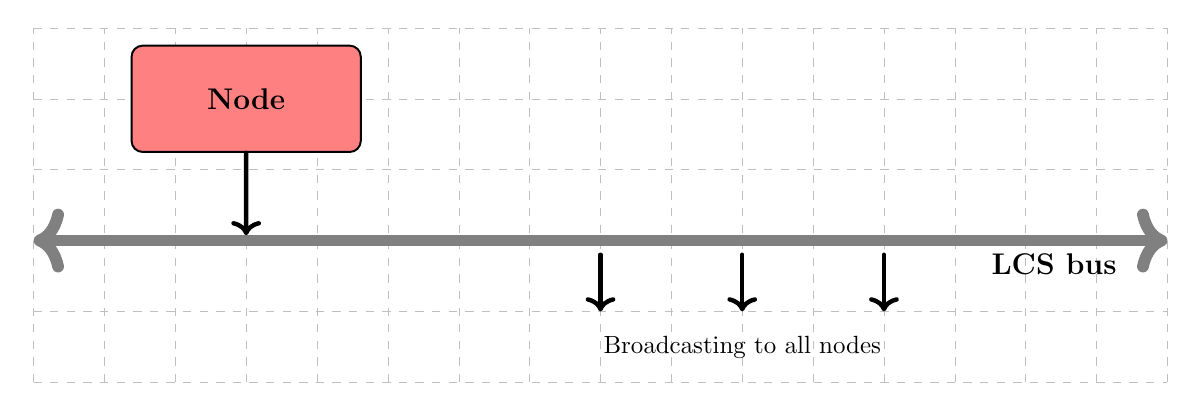
\begin{tikzpicture} [scale=0.9, transform shape]

        \draw[help lines, gray!50, dashed] (0,0) grid(16,5);

         % Thick horizontal line (LCS bus) with text
         \draw[line width=1.5mm, <->, line cap=round, draw=gray, name path=lcsline] 
         (0,2) -- (16,2)
         node[pos= 0.9, tsLargeBold, below] {LCS bus};

          % Define a node
        \node[  tsRoundedRectangle, 
        minimum width=3cm,
        minimum height=1.5cm,
        text width=3cm,
        text centered,
        fill=red!50] (n) at (3,4) {Node};

         % Connecting arrows to LCS bus
        \path[name path=p1] (n.south) -- (3,2); % Define arrow path
        \path[name intersections={of=lcsline and p1, by=intpoint1}];
        \coordinate (adjustedPoint1) at ($(intpoint1) + (0,0.75mm)$);
        \draw[->, ultra thick, line cap=round] (n.south) -- (adjustedPoint1);

        \draw[->, ultra thick, line cap=round] (8, 1.8) -- (8, 1);
        \draw[->, ultra thick, line cap=round] (10, 1.8) -- (10, 1);
        \draw[->, ultra thick, line cap=round] (12, 1.8) -- (12, 1);

        \node at ( 10,0.5) {Broadcasting to all nodes};

    \end{tikzpicture}
\end{center}

All nodes communicate via the layout control bus by broadcasting messages. Every node can send a message, and every node receives the message broadcasted. There is no central master. Since all nodes receive all messages, a node needs to decide whether to react to a message or not. General management and emergency type messages are handled by all nodes. A reply to a specific request will only be handled by the requesting node. The layout control system defines a fairly large set of messages, which can be grouped into several categories:

\begin{smallGapItemize}
    \item General management
    \item Node and Port management
    \item Event management
    \item DCC Track management
    \item DCC Locomotive Decoder management
    \item DCC Accessory Decoder management
    \item RailCom DCC Packet management
    \item Raw DCC Packet management
    \item Firmware Update management
\end{smallGapItemize}

The current implementation is using the CAN bus, which ensures by definition that a message is correctly transmitted. However, it does not guarantee that the receiver actually processed the message. For critical messages, a request-reply scheme is implemented on top. Also, to address possible bus congestion, a priority scheme for messages is implemented to ensure that each message has a chance for being transmitted.

A message is a data packet of up to 8 bytes. The first byte represents the operation code. It encodes the length of the entire packet and opcode number. The first 3 bits represent the length of the message, the remaining 5 bits represent the opCode. For a given message length, there are 32 possible opcode numbers. The last opcode number in each group, 0x1F, is reserved for possible extensions of the opcode number range. The remaining bytes are the data bytes, and there can be zero to seven bytes. 

The message format is independent of the underlying transport method. If the bus technology were replaced, the payload would still be the same. For example, an Ethernet gateway could send those messages via the UDP protocol. The messages often contain 16-bit values. They are stored in two bytes, the most significant byte first and labeled ``xxx-H'' in the message descriptions to come. The message format shown in the tables of this chapter just presents the opCode mnemonic. The actual value can be found in the core library include file.

The byte fields names in an LCS message are explained in greater detail when we discuss the runtime library. For this chapter, the term \texttt{npId-x} will refer to node/port/channel identifier. A node/port/channel identifier is a 16-bit word which consists of the 8-bit nodeId, the 4-bit portId and the 4-bit channel Id. The npId with a portId and channelId of zero will refer to the node itself. The term \texttt{sId} refers to a locomotive session. The remaining message field names, such as \texttt{UID} or \texttt{spDir} or \texttt{argN}are fairly self-explaining.

\section{General Management}

The general management message group contains commands for dealing with the layout system itself. The reset command \texttt{(RESET)} directs all hardware modules, a node, or a port on a node to perform a reset. The entire bus itself can be turned on and off \texttt{(BUS-ON, BUS-OFF)}, enabling or suppressing the message flow. Once the bus is off, all nodes wait for the bus to be turned on again. In case of an emergency the \texttt{(E-STOP)} message stops all running engines. The base station broadcasts a \texttt{(SYS-TIME)} message with the layout time, \texttt{(LCS-INFO)} broadcasts general system information on a regular basis. Finally, there are messages for pinging a node \texttt{(PING)}, perform data synchronization operations \texttt{(SYNC)} and request acknowledgement \texttt{(ACK/ERR)}.

\begin{table}[ht!]
    \centering 
    \resizebox{0.9\textwidth}{!}{ 
        \begin{tabular}{|l|l|l|l|l|l|l|l|}
            \hline
            \textbf{Opcode} & \textbf{Data1} & \textbf{Data2} & \textbf{Data3} & \textbf{Data4} & \textbf{Data5} & \textbf{Data6} & \textbf{Data7} \\
            \hline
            RESET & npId-H & npId-L & flags & & & & \\
            BUS-ON & & & & & & & \\
            BUS-OFF & & & & & & & \\
            E-STOP & & & & & & & \\
            SYS-TIME & arg1 & arg2 & arg3 & arg4 & & & \\
            LCS-INFO & arg1 & arg2 & arg3 & arg4 & & & \\
            PING & npId-H & npId-L & & & & & \\
            ACK & npId-H & npId-L & & & & & \\
            ERR & npId-H & npId-L & code & arg1 & arg2 & & \\
            \hline
        \end{tabular}
    }
\end{table}

\section{Node Id Setup}

When a hardware module is powered on, the first task is to establish the node Id in order to broadcast and receive messages. The \texttt{(REQ-NID)} and \texttt{(REP-ID)} messages are the messages used to implement the protocol for establishing the nodeId. More on this in the chapter on message protocols. A virgin node has the hardware module-specific node type and a node Id of \texttt{NIL} also be set directly through the \texttt{(SET-NID)} command. This is typically done by a configuration tool.

\begin{table}[ht!]
    \centering 
    \resizebox{0.9\textwidth}{!}{ 
        \begin{tabular}{|l|l|l|l|l|l|l|l|}
            \hline
            \textbf{Opcode} & \textbf{Data1} & \textbf{Data2} & \textbf{Data3} & \textbf{Data4} & \textbf{Data5} & \textbf{Data6} & \textbf{Data7} \\
            \hline
            REQ-NID & nId-H & nId-L & nUID-4 & nUID-3 & nUID-2 & nUID-1 & flags \\
            REP-NID & nId-H & nId-L & nUID-4 & nUID-3 & nUID-2 & nUID-1 & flags \\
            SET-NID & nId-H & nId-L & nUID-4 & nUID-3 & nUID-2 & nUID-1 & flags \\
            NCOL    & nId-H & nId-L & nUID-4 & nUID-3 & nUID-2 & nUID-1 & \\
            \hline
        \end{tabular}
    }
\end{table}

All nodes monitor the message flow to detect a potential node collision. This could be for example the case when a node from one layout is installed in another layout. When a node detects a collision, it will broadcast the \texttt{(NCOL)} message and enter a halt state. Manual interaction is required. A node can be restarted with the \texttt{(RES-NODE)} command, given that it still reacts to messages on the bus. All ports on the node will also be initialized. In addition a specific port on a node can be initialized. The hardware module replies with an \texttt{(ACK)} message for a successful node Id and completes the node Id allocation process. As the messages hows, node and port ID are combined. LCS can accommodate up to 4095 nodes, each of which can host up to 15 ports. A Node ID 0 is the NIL node. Depending on the context, a port Id of zero refers all ports on the node or just the node itself.

\section{Node and Port Attributes}

The query node \texttt{(NODE-GET)} and node reply messages \texttt{(NODE-REP)} are available to obtain attribute data from the node or port. The \texttt{(NODE-SET)} allows to set attributes for a node or port for the targeted node. Items are numbers assigned to a data location or an activity. There are reserved items such as getting the number of ports, or setting an LED. In addition, the firmware programmer can also define items with node specific meaning. The firmware programmer defined items are accessible via the \texttt{(NODE-REQ)} and \texttt{(NODE-REP)} messages.

\begin{table}[ht!]
    \centering 
    \resizebox{0.9\textwidth}{!}{ 
        \begin{tabular}{|l|l|l|l|l|l|l|l|}
            \hline
            \textbf{Opcode} & \textbf{Data1} & \textbf{Data2} & \textbf{Data3} & \textbf{Data4} & \textbf{Data5} & \textbf{Data6} & \textbf{Data7} \\
            \hline
            NODE-GET & npId-H & npId-L & item & arg1-H & arg1-L & arg2-H & arg2-L \\
            NODE-SET & npId-H & npId-L & item & val1-H & val1-L & val2-H & val2-L \\
            NODE-REQ & npId-H & npId-L & item & arg1-H & arg1-L & arg2-H & arg2-L \\
            NODE-REP & npId-H & npId-L & item & arg1-H & arg1-L & arg2-H & arg2-L \\
            \hline
        \end{tabular}
    }
\end{table}

Nodes do not react to configuration type messages when in operations mode. To configure a node, the node needs to be put into configuration mode. The \texttt{(OPS)} and \texttt{(CFG)} commands are used to put a node into configuration mode or operation mode. Not all messages are supported in operations mode and vice versa. For example, to set a new nodeId, the node first needs to be put in configuration mode. During configuration mode, no operational messages are processed.

\begin{table}[ht!]
    \centering 
    \resizebox{0.9\textwidth}{!}{ 
        \begin{tabular}{|l|l|l|l|l|l|l|l|}
            \hline
            \textbf{Opcode} & \textbf{Data1} & \textbf{Data2} & \textbf{Data3} & \textbf{Data4} & \textbf{Data5} & \textbf{Data6} & \textbf{Data7} \\
            \hline
            OPS & npId-H & npId-L & & & & & \\
            CFG & npId-H & npId-L & & & & & \\
            \hline
        \end{tabular}
    }
\end{table}

\section{Event Management}

The event management group contains the messages to configure the node event map and messages to broadcast an event and messages to read out event data. The (SET-NODE) with the item value to set and remove an event map entry from the event map is used to manage the event map. An inbound port can register for many events to listen to, and an outbound port will have exactly one event to broadcast. Ports and Events are numbered from 1 onward. When configuring, the portId \texttt{NIL} has a special meaning in that it refers to all portIds on the node.

\begin{table}[ht!]
    \centering 
    \resizebox{0.9\textwidth}{!}{ 
        \begin{tabular}{|l|l|l|l|l|l|l|l|}
            \hline
            \textbf{Opcode} & \textbf{Data1} & \textbf{Data2} & \textbf{Data3} & \textbf{Data4} & \textbf{Data5} & \textbf{Data6} & \textbf{Data7} \\
            \hline
            EVT-ON & npId-H & npId-L & evId-H & evId-L & & & \\
            EVT-OFF & npId-H & npId-L & evId-H & evId-L & & & \\
            EVT & npId-H & npId-L & evId-H & evId-L & arg-H & arg-L & \\
            \hline
        \end{tabular}
    }
\end{table}

\section{DCC Track Management}

Model railroads run on tracks. Imagine that. While on a smaller layout, there is just the track, the track on a larger layout is typically divided into several sections, each controlled by a track node \textnormal{(centralized node or decentralized port)}. The system allows to report back the track sections status \textnormal{(in terms of occupied, free, and detecting the number of engines currently present)}. This function is implemented via the get and set attribute messages. In addition, there are messages to turn on and off the entire tracks.

\begin{table}[ht!]
    \centering 
    \resizebox{0.9\textwidth}{!}{ 
        \begin{tabular}{|l|l|l|l|l|l|l|l|}
            \hline
            \textbf{Opcode} & \textbf{Data1} & \textbf{Data2} & \textbf{Data3} & \textbf{Data4} & \textbf{Data5} & \textbf{Data6} & \textbf{Data7} \\
            \hline
            TON & npId-H & npId-L & & & & & \\
            TOF & npId-H & npId-L & & & & & \\
            \hline
        \end{tabular}
    }
\end{table}

\section{DCC Locomotive Decoder Management}

Locomotive management comprises the set of messages that the base station uses to control the running equipment. To control a locomotive, a session needs to be established \texttt{(REQ-LOC)}. This command is typically sent by a cab handheld and handled by the base station. The base station allocates a session and replies with the \texttt{(REP-LOC)} message that contains the initial settings for the locomotive speed and direction. \text{(REL-LOC)} closes a previously allocated session. The base station answers with the \texttt{(REP-LOC)} message. The data for an existing DCC session can requested with the \texttt{(QRY-LOC)} command. Data about a locomotive in a consist is obtained with the \texttt{(QRY-LCON)} command. In both cases the base station answers with the \texttt{(REP-LOC)} message.

\begin{table}[ht!]
    \centering 
    \resizebox{0.9\textwidth}{!}{ 
        \begin{tabular}{|l|l|l|l|l|l|l|l|}
            \hline
            \textbf{Opcode} & \textbf{Data1} & \textbf{Data2} & \textbf{Data3} & \textbf{Data4} & \textbf{Data5} & \textbf{Data6} & \textbf{Data7} \\
            \hline
            REQ-LOC & adr-H & adr-L & flags & & & & \\
            REP-LOC & sId & adr-H & adr-L & spDir & fn1 & fn2 & fn3 \\
            REL-LOC & sId & & & & & & \\
            QRY-LOC & sId & & & & & & \\
            QRY-LCON & conId & index & & & & & \\
            \hline
        \end{tabular}
    }
\end{table}

Once the locomotive session is established, the \texttt{(SET-LSPD)}, \texttt{(SET-LMOD)}, \texttt{(SET-LFON)}, \texttt{(SET-LOF)} and \texttt{(SET-FGRP)} are the commands sent by a cab handheld and executed by the base station to control the locomotive speed, direction and functions. \texttt{(SET-LCON)} deals with the locomotive consist management and \texttt{(KEEP)} is sent periodically to indicate that the session is still alive. The locomotive session management is explained in more detail in a later chapter when we talk about the base station.

\begin{table}[ht!]
    \centering 
    \resizebox{0.9\textwidth}{!}{ 
        \begin{tabular}{|l|l|l|l|l|l|l|l|}
            \hline
            \textbf{Opcode} & \textbf{Data1} & \textbf{Data2} & \textbf{Data3} & \textbf{Data4} & \textbf{Data5} & \textbf{Data6} & \textbf{Data7} \\
            \hline
            SET-LSPD & sId & spDir & & & & & \\
            SET-LMOD & sId & flags & & & & & \\
            SET-LFON & sId & fNum  & & & & & \\
            SET-LFOF & sId & fNum  & & & & & \\
            SET-FGRP & sId & fGrp  & data & & & & \\
            SET-LCON & sId & conId & flags & & & & \\
            KEEP & sId & & & & & & \\
            \bottomrule
        \end{tabular}
    }
\end{table}

Locomotive decoders contain configuration variables too. They are called CV variables. The base station node supports the decoder CV programming on a dedicated track with the \texttt{(REQ-CVS)}, \texttt{(REP-CVS)} and \texttt{(SET-CVS)} messages. The \texttt{(SET-CVM)} message supports setting a CV while the engine is on the main track. \texttt{(DCC-ERR)} is returned when an invalid operation is detected.

\begin{table}[ht!]
    \centering 
    \resizebox{0.9\textwidth}{!}{ 
        \begin{tabular}{|l|l|l|l|l|l|l|l|}
            \hline
            \textbf{Opcode} & \textbf{Data1} & \textbf{Data2} & \textbf{Data3} & \textbf{Data4} & \textbf{Data5} & \textbf{Data6} & \textbf{Data7} \\
            \hline
            SET-LSPD & sId & cv-H & cv-L & mode & val & & \\
            REQ-CVS  & cv-H & cv-L & mode & val & & & \\
            REP-CVS  & cv-H & cv-L & val  & & & & \\
            SET-CVS  & cv-H & cv-L & mode & val & & & \\
            \hline
        \end{tabular}
    }    
\end{table}

The SET-CVM command allows to write to a decoder CV while the decoder is on the main track. Without the RailCom channel, CVs can be set but there is not way to validate that the operation was successful.

\section{DCC Accessory Decoder Management}

Besides locomotives, the DCC standards defines stationary decoders, called accessories. An example is a decoder for setting a turnout or signal. There is a basic and an extended format. The \texttt{(SET-BACC)} and \texttt{(SET-EACC)} command will send the DCC packets for stationary decoders. Similar to the mobile decoders, there are POM / XPOM messages to access the stationary decoder via RailCom capabilities.

\begin{table}[ht!]
    \centering 
    \resizebox{0.9\textwidth}{!}{ 
        \begin{tabular}{|l|l|l|l|l|l|l|l|}
            \hline
            \textbf{Opcode} & \textbf{Data1} & \textbf{Data2} & \textbf{Data3} & \textbf{Data4} & \textbf{Data5} & \textbf{Data6} & \textbf{Data7} \\
            \hline
            SET-BACC & adr-H & adr-L & flags & & & & \\
            SET-EACC & adr-H & adr-L & val & & & & \\
            \hline
        \end{tabular}
    }
\end{table}

These commands are there for completeness of the DCC control interfaces. There could be devices that are connected via the DCC track that we need to support. However, in a layout control system the setting of turnouts, signals and other accessory devices are more likely handled via the layout control bus messages and not via DCC packets to the track. This way, there is more bandwidth for locomotive decoder DCC packets.

\section{RailCom DCC Packet management}

With the introduction of the RailCom communication channel, the decoder can also send data back to a base station. The DCC POM and XPOM packets can now not only write data but also read out decoder data via the RailCom back channel. The following messages allow to send the POM / XPOM DCC packets and get their RailCom based replies.

\begin{table}[ht!]
    \centering 
    \resizebox{0.9\textwidth}{!}{ 
        \begin{tabular}{|l|l|l|l|l|l|l|l|}
            \hline
            \textbf{Opcode} & \textbf{Data1} & \textbf{Data2} & \textbf{Data3} & \textbf{Data4} & \textbf{Data5} & \textbf{Data6} & \textbf{Data7} \\
            \hline
            SET-MPOM & sId & ctrl & arg1 & arg2 & arg3 & arg4 & \\
            REQ-MPOM & sId & ctrl & arg1 & arg2 & arg3 & arg4 & \\
            REP-MPOM & sId & ctrl & arg1 & arg2 & arg3 & arg4 & \\
            SET-APOM & adr-H & adr-L & ctrl & arg1 & arg2 & arg3 & arg4 \\
            REQ-APOM & adr-H & adr-L & ctrl & arg1 & arg2 & arg3 & arg4 \\
            REP-APOM & adr-H & adr-L & ctrl & arg1 & arg2 & arg3 & arg4 \\
            \hline
        \end{tabular}
    }
\end{table}

The XPOM messages are DCC messages that are larger than what a CAN bus packet can hold. With the introduction of DCC-A such a packet can hold up to 15 bytes. The LCS messages therefore are sent in chunks with a frame sequence number and it is the responsibility of the receiving node to combine the chunks to the larger DCC packet.

\section{Raw DCC Packet Management}

The base station allows to send raw DCC packets to the track. The \texttt{(SEND-DCC3)}, \texttt{(SEND-DCC4)}, \texttt{(SEND-DCC5)} and \texttt{(SEND-DCC6)} are the messages to send these packets. Any node can broadcast such a message, the base station is the target for these messages and will just send them without further checking. So you better put the DCC standard document under your pillow.

\begin{table}[ht!]
    \centering 
    \resizebox{0.9\textwidth}{!}{ 
        \begin{tabular}{|l|l|l|l|l|l|l|l|}
            \hline
            \textbf{Opcode} & \textbf{Data1} & \textbf{Data2} & \textbf{Data3} & \textbf{Data4} & \textbf{Data5} & \textbf{Data6} & \textbf{Data7} \\
            \hline
            SEND-DCC3 & arg1 & arg2 & arg3 & & & & \\
            SEND-DCC4 & arg1 & arg2 & arg3 & arg4 & & & \\
            SEND-DCC5 & arg1 & arg2 & arg3 & arg4 & arg5 & & \\
            SEND-DCC6 & arg1 & arg2 & arg3 & arg4 & arg5 & arg6 & \\
            \hline
        \end{tabular}
    }
\end{table}

The above messages can send a packet with up to six bytes. With the evolving DCC standard, larger messages have been defined. The XPOM DCC messages are a good example. To send such a large DCC packet, it is decomposed into up to four LCS messages. The base station will assemble the DCC packet and then send it. 

\begin{table}[ht!]
    \centering 
    \resizebox{0.9\textwidth}{!}{ 
        \begin{tabular}{|l|l|l|l|l|l|l|l|}
            \hline
            \textbf{Opcode} & \textbf{Data1} & \textbf{Data2} & \textbf{Data3} & \textbf{Data4} & \textbf{Data5} & \textbf{Data6} & \textbf{Data7} \\
            \hline
            SEND-DCCM & ctrl & arg1 & arg2 & arg3 & arg4 & & \\
            \hline
        \end{tabular}
    }
\end{table}

\section{DCC errors and status}

Some DCC commands return an acknowledgment or an error for the outcome of a DCC subsystem request. The \texttt{(DCC-ACK)} and \texttt{(DCC-ERR)} messages are defined for this purpose.

\begin{table}[ht!]
    \centering 
    \resizebox{0.9\textwidth}{!}{ 
        \begin{tabular}{|l|l|l|l|l|l|l|l|}
            \hline
            \textbf{Opcode} & \textbf{Data1} & \textbf{Data2} & \textbf{Data3} & \textbf{Data4} & \textbf{Data5} & \textbf{Data6} & \textbf{Data7} \\
            \hline
            DCC-ACK & & & & & & & \\
            DCC-ERR & code & arg1 & arg2 & & & & \\
            \hline
        \end{tabular}
    }
\end{table}

\section{Analog Engines}

The messages defined for the DCC locomotive session management as outlined above are also used for the analog engines. An analog engine will just like its digital counterpart have an allocated locomotive session and the speed/dir command is supported. All other commands will of course not be applicable. The speed/dir command will be sent out on the bus and whoever is in control of the track section where the analog engine is supposed to be, will manage that locomotive. In the following chapters we will answer the question of how exactly multiple analog engines can run on a layout.

\section{Firmware Update Management}

LCS supports a method for updating the firmware remotely. This involves loading a new firmware image. A typical approach is to split the available program memory in two partitions and load the new image in the non-active partition. When the firmware is transmitted and valid, the next restart will boot using the new firmware. There is a whole chapter later in the book about the firmware update.

\begin{table}[ht!]
    \centering 
    \resizebox{0.9\textwidth}{!}{ 
        \begin{tabular}{|l|l|l|l|l|l|l|l|}
            \hline
            \textbf{Opcode} & \textbf{Data1} & \textbf{Data2} & \textbf{Data3} & \textbf{Data4} & \textbf{Data5} & \textbf{Data6} & \textbf{Data7} \\
            \hline
            START-LOAD & npId-H & npId-L & cmd & size-1 & size-2 & size-3 & size-4 \\
            START-BLOCK & npId-H & npId-L & cmd & blockId-H & blockId-L & & \\
            SEND-DATA & npId-H & npId-L & cmd & data1 & data2 & data3 & data4 \\
            END-BLOCK & npId-H & npId-L & cmd & blockId-H & blockId-L & chkSum-H & chkSum-L \\
            END-LOAD & npId-H & npId-L & cmd & chkSum-1 & chkSum-2 & chkSum-3 & chkSum-4 \\
            \hline
        \end{tabular}
    }
\end{table}

A firmware update starts with the \texttt{(START-LOAD)} message. The transfer uses the \texttt{(START-BLOCK)}, \texttt{(SEND-DATA)} and \texttt{(END-BLOCK)} messages to transmit a block. Each block is validated with a 16-bit checksum. The \texttt{(END-LOAD)} message completes the download, the entire image is checked against a 32-bit checksum.


\section{Summary}

This chapter introduced the general message formats for the layout control bus functions and how they are used in the LCS protocols. The message format is built upon an 8-byte message format that is suitable for the industry standard CAN bus. Although there are many other standards and communication protocols, the CAN bus is a widely used and robust bus. Since all data is encoded in the message, there is no reason to select another communication media. But right now, it is CAN. The next chapter will now concentrate on the message protocols.
 
\input{part-concepts//chapter-lcs-concepts-message-protocols} 
\input{part-concepts//chapter-lcs-concepts-dcc-subsystem}
\input{part-concepts//chapter-lcs-concepts-analog-subsystem}
\chapter{Hardware Modules}

talk a little about the modules and extensions ...

we will have a main board and extension boards

main board hosts the controller and perhaps special HW that needs to be close to the controller

they will always have the LCS bus interface and a power supply for itself and the extentions

extensions are access via a I2C bus

they implement functions for as sensors and actors

there is a standardized interface connector between main board and extension boards

up to 4 extension boards can be connected to a main board




\chapter{Sensors and Actors}

Sensors and Actors are the eyes, ears and hands for any layout system. The requirements and options are numerous and the list of desired features needed is perhaps never complete. Sensors, the eyes and ears, are mainly the event producers. A block occupancy detection, a power overload detection, but also a push of a button on a layout control panel are good examples. The counterpart to sensors  are actors. Actors, the hands, are the family of LCS nodes and special hardware that control turnouts, signals and whatever else there is. This chapter will present the most common actors and sensor nodes found on a layout. Building upon the concept of main controller, base station, block controller and extensions board concepts, this part of the book will present how the pieces that make up a node can be put together from the basic building blocks.

With so many sensors and actors, a key requirement is to implement a concept where most of the functional parts can be used in different combinations. The chapter on hardware design already presented the main controller and extensions concept. A key reason for this concept were exactly the large variety of sensors and actors.

\begin{itemize}
\item main controller
\item block controller
\item base station
\end{itemize}

The main controller portion, common to all, will feature the processor, the message interface for the LCS bus, and the power supply for the board and the extensions. Some LCS nodes need a larger NVM storage. The main controller board will allow an optional installation of a NVM chip. Furthermore, the power supply, intended for generating the power for main controller board as well as the VCC power for the extensions, will also feature an optional installation of power failure detection. Before going into the detailed extension board designs, what boards would be need? Here is a brief look ahead of the boards to come.
\begin{itemize}
\item \textbf{Occupancy Detector}. The occupancy detector extension board is a companion to the block controller board. It will offer 4 channels, i.e. tracks that match the block controller output, with a set of detectors on each channel.
\item \textbf{Turnout}. The turnout extension board features a set of turnouts with frog polarization. Similar to the occupancy detector the boards is designed to go with the block controller board.
\item \textbf{Servo}. The servo extension board is a universal board, which can be connected to any controller board presented. It features a set of general servo outputs.
\item \textbf{GPIO}. The GPIO extension boards is a universal digital input / output board. It is typically used for input such as switches or push buttons a well as LEDs connected. Care has to be taken to match the the number of output consumers with the what the individual output pins can drive.
\item \textbf{Signal}. The signal extension bard is another general purpose board designed for driving the LED equipped signals. It is able to not only match the power requirements but also allow for dimming and / or blinking the individual lights.
\item \textbf{Relays}. The relay extension board is a general purpose board intended to drive a set of relays. The relays, which are not part of the board, can be driven with different voltage levels.
\item \textbf{Cab Control}. The cab handhelds as well as stationary cab control devices are also just an extension. There is no reason why this extension could for example not be connected to a base station and build a complete control station fort a smaller layout.
\item \textbf{Prototyping}. It is often useful to just do a quick sketch of a function desired for an extension board. So, how about an extension board with the extension address resolution logic and just room for building your own HW designs.
\end{itemize}

Extension boards implements the hardware for the particular sensor or actor type. All extension boards need to feature the connectors, so that more than one extension board can share the same controller board. However, only the first board will benefit from the availability of all extension bus signal lines. It is not a requirement that the second extension board will get the same signals. It is also not a requirement that an extension board does have the decoding logic described in the extension hardware design chapter. For example, the power module unit which together with main controller is a base station, does not have that logic. It expects to be connected directly to the main controller board. The power module board will however still route power, DCC and I2C signals. The I2C bus plays a key role in communicating with an I2C type extension board. Each I2C based extension board will have the extension board decoding logic, which is essential for proper addressing that board.
\input{part-concepts//chapter-lcs-concepts-summary}
    %--------------------------------------------------------------------------------
%
% 
%--------------------------------------------------------------------------------
\part{LCS Core Layer}

 \input{part-core-layer/chapter-runtime-lib/chapter-runtime-lib}
 \input{part-core-layer/chapter-runtime-lib-command-interface/chapter-runtime-lib-command-interface}
 \input{part-core-layer/chapter-runtime-lib-example/chapter-runtime-lib-example}
 \input{part-core-layer/chapter-controller-dependent-codechapter-controller-dependent-code} 
 \chapter*{UI Elements}
\addcontentsline{toc}{chapter}{UI Elements}

User interfaces such as Cab Handhelds or Switch Panels offer the user control and display elements for a layout. Typically there many buttons and LEDs but also rotary encoders and displays. You start an Arduino project and the first Led is blinking, a button is pushed. Before you know it, buttons need to be debounced, short and long pressed, active high or active low. You would like to toggle a Led and remember its state. There are displays with different interfaces and capabilities. On some displays you want to control the brightness and contrast. Finally, in some projects you run out of physical pins and want to connect an array of buttons or LEDs through a shift register. The list is long. In all Arduino projects you implement it somehow directly in project just to take part of the functions to the next project and so on. UI Elements is the library the implements the most common UI elements.

\section*{Concpets}
\addcontentsline{toc}{section}{Concepts}

When building simple controller applications, a LED and a button are the most common things used in becoming familiar how to program for such a controller. Digital pins configured as an output and the LED will light up when driven by the output pin. Likewise, a HW pin configured as an input the state of a button can be read. But wait, while LEDs are electronic items, a button is something mechanical and pushing it typically will cause the value read to initially "bounce" between low and high. The first thing the UI Elements library will do is to shield the user from these mechanical issues.

Furthermore a button can be pushed once, double or for a longer period. The UI Elements library works with a state machine approach. A periodic function, "tick" is expected to be called from the outer loop of the program. For all UI Element Objects, the state machine is called and the element state is advanced. Communication back to the program is handled via previously registered callback functions.

Displays come in a large variety and capabilities. UI Elements will offer an abstraction of an ASCII display with a fixed number of line and columns. LCD and OLED displays are unified with with a simple interface to set a cursor and to write a character to that position.

Finally, buttons and LEDs can be combined to arrays. Consider a Cab Handheld with for example 10 buttons, a rotary encoder, several LEDs and a display. We will quickly run out of HW pins on the controller. An array of buttons features the same capabilities of a single button object, the values of the buttons are however read in through a shift register serial output or a PIO Extender chip, such as we used for actors and sensors before, are required.

\section{Buttons}

A button is an object that has one input value and analyzes whether the button was clicked, double clicked or long pressed. All this is done with a state machine that manages the button state. For each action a callback function can be registered. There is also a callback function for getting the button data. Buttons are one  of the most used UI Elements. This set of methods implements the single button and an array of buttons. Each button is essentially a state machine with a set of defined callback functions. The time for debouncing, detecting a click or a long press can be set individually for each button. A switch is also just a button with a long press characteristic. For each button a button descriptor keeps the data about callback, HW pin and so on. The following brief example shows how to implement a single button and handle the click event. The following example shows a simple button clicked implementation.

// ??? rather have an abstract picture, it is early in the book ...

\lstset{language=c++, style=codesnippetstyle}
\begin{lstlisting}
#include "UIElements.h"

// create the button, pin 5 is the button input
UIButton aButton( 5 );

bool getButtonData( uint8_t pin ) {

	return( digitalread( pin ));
}

void buttonHandler( uint8_t buttonId ) {

	// the button was clicked. 
	// buttonId contains the pin number 5
}

void setup ( ) {

	// the setup function, register the click callback
	aButton.attachgetDataFunction( getButtonData );
	aButton.attachButtonClicked( buttonHandler );
}

void loop ( ) {

    // in the main loop of the program the UIElements "tick" function.
	UIElements::tick( );
}

\end{lstlisting}
\FloatBarrier

Instead of implementing the button data retrieval directly in the button object, there is a callback that obtains the hardware value. This might look like an overkill in abstracting a button. But consider a button connected to a serial shift register or a button connected to an interface chip such as the MCP23017. Each of these hardware interfaces would require a special case in the button object. Abstracting the data retrieval, allows to implement very different hardware buttons. All this comfort comes with a price though. The button object has a size of roundabout 26 to 32 bytes. So, an array of 256 buttons would occupy quite some memory storage. For such applications, a dedicated special button array class would perhaps be the better choice. Note that the buttonId does not necessarily have to be a physical pin number. For example, a shift register with implementation with 64 buttons could simply assign logical numbers that the data retrieval function understands to get the correct bit from the shift register.

\section{Rotary Encoders}

A rotary encoder works similar to a button. It is a type of position sensor that generates an electrical signal according to the rotational movement. The most common one has two outputs that are turned on 90 degrees out of phase from each other. Just monitoring one of the inputs allows for detecting rotary movement. However, analyzing both inputs at the same time allows for detecting the rotational direction. If the pin A changes its signal level, examining the input B allows for determining the direction. If both inputs signals are equal the rotation is clockwise, else counter clock wise. The UIEncoder element manages all these details and offers a callback to be invoked when the position of the rotary encoder changes. Just like buttons, there is a data retrieval callback function. Here is a simple example.

// ??? rather have an abstract picture, it is early in the book ...


\lstset{language=c++, style=codesnippetstyle}
\begin{lstlisting}
#include "UIElements.h"

// create the rotary encoder, pin 5 and 6 are the inputs, 
// MIN and MAX defines the encoder range.
UIEncoder anEncoder( 5, 6, MIN, MAX );

bool getEncoderData( uint8_t pin ) {

	return( digitalRead( pin ));
}

void positionChangedHandler( uint8_t newPosition ) {

	// the encoder was turned, the delta passed to the callback function.
}

void setup ( ) {
	
	// the setup function 
	// register the positionChanged callback
	anEncoder.attachGetDataFunction( getEncoderData );
    anEncoder.attachPositionChanged( positionChangedHandler );
}

void loop ( ) {

    // in the main loop of the program the UIElements "tick" function.
	UIElements::tick( );
}
\end{lstlisting}
\FloatBarrier

\section{LEDs}

When talking about buttons and switches, the LEDs built the counterpart and signal a state. A LED is an object that can be turn on and off and blink. Just like buttons a state machine manages the LED state and there is a callback for setting the data according to the hardware implementation.

\section{Displays}

In addition to a LED signaling light, there is the requirements to display human readable text. The UI element display is an object that represents a matrix of ASCII characters. A display has n lines with m characters. There are methods to set a cursor to a line / column position and a method to print a character. There is a variety of display hardware available. The common ones are a LCD display with 4 x 20 or 2 x 16 characters. There are also OLED displays which are graphical displays with for example 128 x 64 pixels. These display can print characters using different fonts.

The display UI element provides as a common function set the methods to clear a display, set a cursor position and write a character to that position. In addition, each type of display has capabilities specific to this display. A LCD display has methods for turning on and off the backlight. There are also blinking cursors and so on. The OLED display allows for smaller or larger character fonts. While the display UI element object presents a common method set for all display types it will not shield these additional capabilities. The following shot example will show an OLED display connected via the default I2C lines.

// ??? rather have an abstract picture, it is early in the book ...


\lstset{language=c++, style=codesnippetstyle}
\begin{lstlisting}
#include "UIElements.h"

UIDisplay *oled;

void setup ( ) {

	oled = new UIDisplayOledSSD1306 ( DT_OLED_DISPLAY_128x64_16_4 );

	// write to top of screen
	oled -> clear( );
	oled -> print( "Hello world!");

	// write to line 2
	oled -> setCursor( 0, 2 );
	oled -> print( "Line 2");
}

void loop ( ) {
	// in the main loop of the program the UIElements "tick" function. This is not really
	// necessary for the display function, but for the rest of UI elements.
	UIElements::tick( );
}
\end{lstlisting}
\FloatBarrier

\section{Screens}

UI Elements such as Buttons, Knobs, LEDs and displays are the atoms of a user interface. The next level is to organize these atoms into screens. A screen is first of all a display UI element that is manipulated with the help of UI input elements such as buttons. The UI Screen is a very simple element to organize and manipulate these screens.

The UIScreen object is the class for implementing a screen. Screens are a display of whatever you want to put on that display.There are virtual methods that will be called when a button event such a click is encountered. Two buttons needed for navigation. They are the MENU and SELECT button. With the exception of the root screen, a screen has a parent and a potential child list. The hierarchy is formed by appending a screen to another screen child list. The MENU button is typically used to scroll through the child list. A long press of the menu button always gets back to the root screen's first child, no matter where you are. Child lists are toggled through with the menu button in a circular fashion. From the last screen on the child list, the next toggle gets us to the first child. The SELCET button selects the current screen and triggers an action. When navigating to a screen, the exit callback is invoked for the screen to leave and the enter callback is invoked for the screen to enter. The exit callback would typically be used to clean up of store data away, the enter callback would be used to set up the data and display the initial screen content.

// ??? rather have an abstract picture, it is early in the book ...


\lstset{language=c++, style=codesnippetstyle}
\begin{lstlisting}
a conceptual picture of a screen hierarchy ?

MENU -> MENU -> MENU -> MENU -> MENU -> back to first menu
  |
  v
SUB-MENU
   |
   v
SUB-MENU
   |
   v
SUB-MENU
  |
  v
  back to first sub menu
\end{lstlisting}
\FloatBarrier

To keep the screen hierarchy flexible, the meaning of the MENU and SELECT button within a given screen is not fixed. But as a convention, the MENU button should be used to toggle through screens, the SELECT button is used to enter a screen child list and also as a kind of commit button. All other buttons, if any are completely user defined.

The connection from UIElement events to screens is handled by registering the static callback functions defined for the UI elements. All UI Elements for which the callback set will just pass the event to the current screen. For example, the UIScreen base class has the MENU and SELECT button event handler to navigate through the screens.

A screen that inherits from the UIScreen could overwrite these handlers and assign a new meaning to the MENU and SELECT button. For the other elements, i.e. the other buttons but also encoders, there are dedicated handlers that are passed the resource ID of UIElement. A screen that for example that displays the value of an encoder UIElement will build a class that inherits form UIScreen and override the encoder callback. In a similar way the MENU and SELECT button can also be override, but then it is up to the implementer to handle the navigation. That's it.

// ??? rather have an abstract picture, it is early in the book ...

// ??? \textbf{note} have an example ...

\section{Summary}

This chapter presented the UI element library, which is the common UI layer for handhelds, control panels and monitor displays.

 \input{part-core-layer/chapter-concepts-firmware-design/chapter-concepts-firmware-design}
    %--------------------------------------------------------------------------------
%
% 
%--------------------------------------------------------------------------------
\part{LCS Hardware}

\input{part-hardware//chapter-lcs-concepts-hardware-main-module-design/chapter-lcs-concepts-hardware-main-module-design}
\input{part-hardware/chapter-lcs-main-controller-hardware-pico}
\input{part-hardware/chapter-lcs-power-module-design}
\input{part-hardware/chapter-lcs-railcom-signal-detector}
\input{part-hardware/chapter-lcs-hardware-part-summary}
    %--------------------------------------------------------------------------------
%
% 
%--------------------------------------------------------------------------------
\part{LCS Base Station}

\input{part-base-station/chapter-base-station-introduction/chapter-base-station-introduction}
\input{part-base-station/chapter-base-station-hardware/chapter-base-station-hardware}
\input{part-base-station/chapter-base-station-firmware/chapter-base-station-firmware}

    %--------------------------------------------------------------------------------
%
% 
%--------------------------------------------------------------------------------
\part{LCS Cab Handheld}

\input{part-cab-handheld/chapter-cab-handheld-introduction/chapter-cab-handheld-introduction}
\input{part-cab-handheld/chapter-cab-handheld-hardware/chapter-cab-handheld-hardware}
\input{part-cab-handheld/chapter-cab-handheld-firmware/chapter-cab-handheld-firmware}

    %--------------------------------------------------------------------------------
%
% 
%--------------------------------------------------------------------------------
\part{LCS Block Controller}

\input{part-block-controller/chapter-concepts-signaling-block-control/chapter-concepts-signaling-block-control}
\chapter{The Block Controller}

// ??? introduction to the block controller topic...

A block controller is an LCS node that can manage one more blocks, each with one or more sections. This chapter will describe the firmware developed for the block controller. The block controller features several ports for the blocks and associated turnouts, signals and so on.

First, each block must be uniquely defined in the layout. A block controller ID consists of the node ID and a portId resenting that block. A layout could have theoretically 4095 nodes with 4 blocks each. In reality, we need nodes also for other purposes, but still this number is large enough even for really large layouts. Let'S first look a t what ports are needed.

\input{part-block-controller/chapter-block-controller-hardware/chapter-block-controller-hardware}
\input{part-block-controller/chapter-block-controller-firmware/chapter-block-controller-firmware}

    %--------------------------------------------------------------------------------
%
% 
%--------------------------------------------------------------------------------
\part{LCS Gateways}

\input{part-gateway/chapter-gateway-module/chapter-gateway-module}

    %--------------------------------------------------------------------------------
%
% 
%--------------------------------------------------------------------------------
\part{LCS Extensions}

\input{part-extensions/chapter-hardware-extension-module-design/chapter-hardware-extension-module-design}
\input{part-extensions/chapter-extension-track-occupancy-detector/chapter-extension-track-occupancy-detector}
\input{part-extensions/chapter-extension-cab-control/chapter-extension-cab-control}
\input{part-extensions/chapter-extension-prototype/chapter-extension-prototype}
    %--------------------------------------------------------------------------------
%
% 
%--------------------------------------------------------------------------------
\part{LCS Utilities}

\input{part-utilities/chapter-lcs-dcc-monitoring/chapter-lcs-dcc-monitoring}
\chapter{Layout Connector Panel}

There are situations where one would connect a mobile node to the LCS bus. A good example is a cab handheld which you would like to plug in close where the session operation currently is. Even though the world moves more and more to wireless, such a connector front panel installed around the layout is not a bad idea. The panel can also be used to feature an emergency stop button and perhaps some rudimentary power status indication.

\section{Requirements}

A layout connector panel needs to provide two connectors for the LCS bus coming in and going out. The signal lines are just routed through with the exception of the power line. While these two connectors are behind the scene at the back of the front panel, two more connectors are exposed via the front panel. These are the connectors where for example a cab handheld would be plugged in. In addition to the two front panel connectors, there is an option to connect an emergency stop button. When pushed, the lines is drawn to ground and all nodes would detect the signal going low.

The power line is not directly routed to the front panel connectors. There should be an option to have an external power supply to provide the power to the nodes. It depends on the total power consumption we expect on the LCS bus. The central source will be a power supply that delivers about one amp to the lCS bus. To power a couple of handhelds or small sensors nodes, would not be a problem. As the power demand grows, a separate power supply such as shown on the schematic below will deliver the necessary power.

\section{Implementation}

The following schematic shows the LCS connector panel schematic. The upper part contains all the connectors and the option to connect an external power source to the front panel. The lower part shows a simple power supply, which could directly be hosted on the connector PCB.

\begin{tikzpicture}[scale=0.9, transform shape]

    \draw[help lines, gray!50, dashed] (0,0) grid( 16,8);
    \node at (8,4) {picture};

\end{tikzpicture}

\section{Summary}

This rather short chapter presented how a layout connector panel could be designed. Such panels are placed on strategic points around the layout. Besides connecting mobile devices to the LCS bus, there is also the option to feed these devices with an external power.  The panel is also a good spot to place emergency stop buttons around the layout.  The current panel is just connector routing panel.  Additional status information for power on, bus activity, and so on could also be put onto such a panel. However, anything more complex would require to put some controller logic on the panel as well.


\input{part-utilities/chapter-lcs-utility-boards/chapter-lcs-utility-boards}
\input{part-utilities/chapter-lcs-firmware-update/chapter-lcs-firmware-update}
    %--------------------------------------------------------------------------------
%
% 
%--------------------------------------------------------------------------------
\part{LCS Configuration}

\input{part-configuration/chapter-lcs-layout-system-configuration}
    %--------------------------------------------------------------------------------
%
% 
%--------------------------------------------------------------------------------
\part{LCS Reference}

??? to do ...
    %--------------------------------------------------------------------------------
%
% 
%--------------------------------------------------------------------------------
\part{Appendix}

 \appendix 

\chapter{Resources}


\section{GitHub Structure}

LCS Nods

LCS Book

\section{Libraries}

\begin{itemize}
\item LcsCdcLib
\item LcsRuntimeLib
\item LcsUIElementsLib
\item LcsExtXXXLib ( one for each extension )
\end{itemize}

\section{External libraries}

can2040

\section{Firmware}

\begin{itemize}
\item LcsBaseStation
\item LcsBlockController
\item LcsCabHandheld
\item LcsCabThrottle
\item LcsMonitor
\end{itemize}

\section{Schematics and Boards}

Schematics and Boards so far

... to fill in ...

\section{About this Book}

how to make it 

structure

\chapter{LCS Nodes and EasyEda}

The schematics and boards shown were all developed using the EasyED software. EasyEDA is a design tool for developing the schematics and PCB layouts. A PCB can then be ordered at very reasonable prices. Even during LCS node early design stages it is therefore sometimes worthwhile to just produce a PCB and avoid searching software bugs that are actually just loose connection on a breadboard. To ease the development, there are experimental boards. However when it comes to a final design, PCB boards need to be developed and ordered in larger quantitates. The LCS Node design introduced contains a main controller board and extension boards. The sizes and location of the connectors have been standardized. This appendix contains the PCB drawings of the most common LCS boards to give you a head start in developing your own boards, ensuring that all boards fit together.

\section{Symbols and Footprints}

EasyEDA allows you to create symbols that represent components and can be placed in a schematic. To each symbol there should be a footprint that is used to put the component on to the PCB. The connection between the two is a list of assignments that associate a \textbf{pin} on the symbol with a \textbf{pad} on the footprint. For LcsNodes there is a list of symbols and footprints to ensure that the PCBs do have all their connectors at the exact place, so that they fit together.

\subsection{Symbols}

To ease the development of LCS boards, the entire board and its connectors are available as a symbol. Depending on the category, the symbol features the connection end points for the connectors found on the board. This symbol is associated with the corresponding footprint described in the next section. Note that the footprint needs to match the symbol. That is the number, position and meaning of the connectors found on the board map, only length of the PCB board varies.

\subsection{Main Controller Board Footprints}

This section contains all the footprints available so far. There are three main categories. The first is anything that represents an LCS Controller portion. There are the connections to the LCS bus and the power input connector. On the left side are two connectors. The upper connector is reserved for up to four tack pow lines. Below is the LCS extension board connector. The basic LCS Main Controller Board for example is the 16cm x 10cm board shown below.

\begin{figure}[htbp]
    \centering
    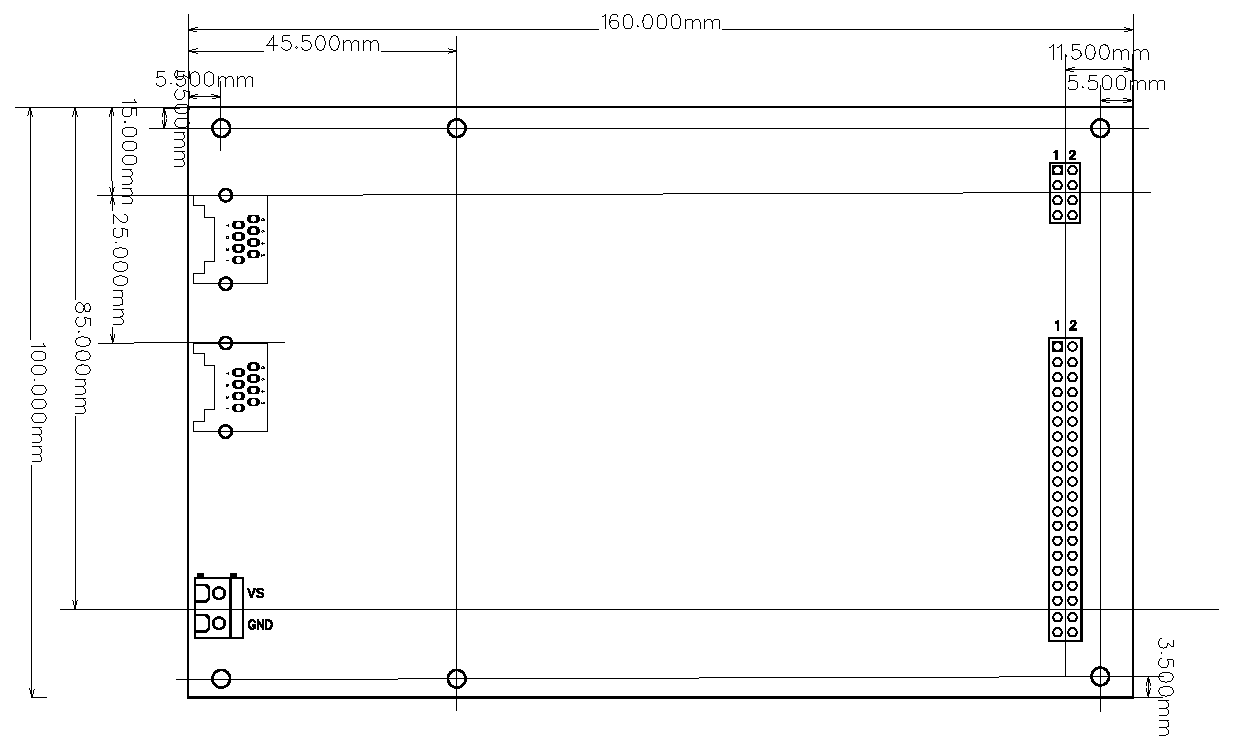
\includegraphics[page=1, scale=0.7]{./Figures/LCS-FP-MAIN-CTRL-10X16.pdf}
    \caption{LCS-FP-MAIN-CTRL-10X16}
    %\label{fig:your-label}
\end{figure}

\FloatBarrier

The mounting holes may look a little odd. As shown in the text to follow, there are extension boards with a form factor of 12cm x 10cm. When are the are mounted on top of the 16cm board, the holes nicely match. 

\section{Extension Boards Footprints}

Next, there are the extension boards. The extension board has the LCS connectors on the left side. The right hand side will typically host the connectors to the layout. These boards can either directly plugged into a controller board or into a bus PCB which hosts controller and more than one extension board. In either case, the extension boards are the same.

\begin{figure}[htbp]
    \centering
    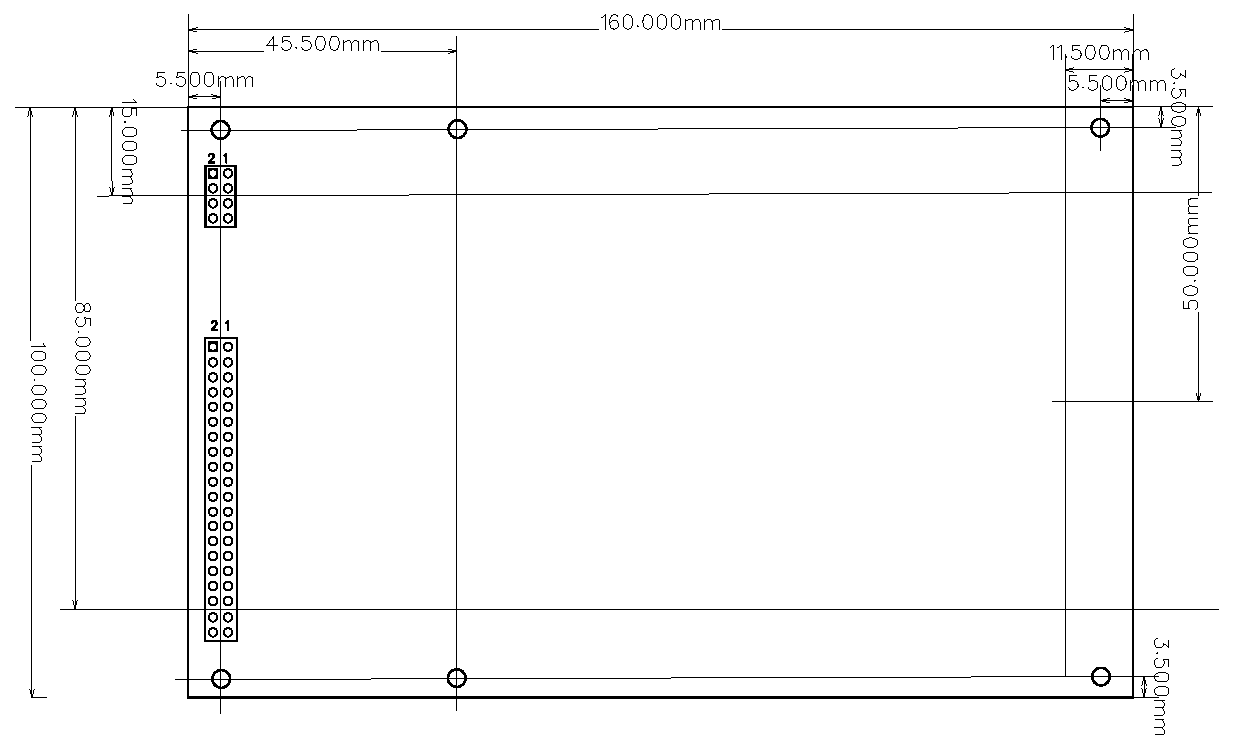
\includegraphics[page=1, scale=0.7]{./Figures/LCS-FP-EXT-L-10X16.pdf}
    \caption{LCS-FP-EXT-R-10X16}
    %\label{fig:your-label}
\end{figure}

\FloatBarrier

In addition to the basic 16cm x 10cm form factor is a set of 12cm x 10cm boards. They have exactly the same layout, except that their length is 12cm instead of 16cm. As always, there could be many more combinations as new boards with different demands are developed. Nevertheless it is important that when connectors are used, that they have the same meaning and are placed at the same location. This is the whole idea of using footprints to ensure this exact fitting.

\section{Pad Numbers}

In EasyEDA, the symbol pads and the PCB pads meet via PAD numbers. Across all symbols and PCBs the numbers assignments are shown in the figure below.

\begin{figure}[htbp]
    \centering
    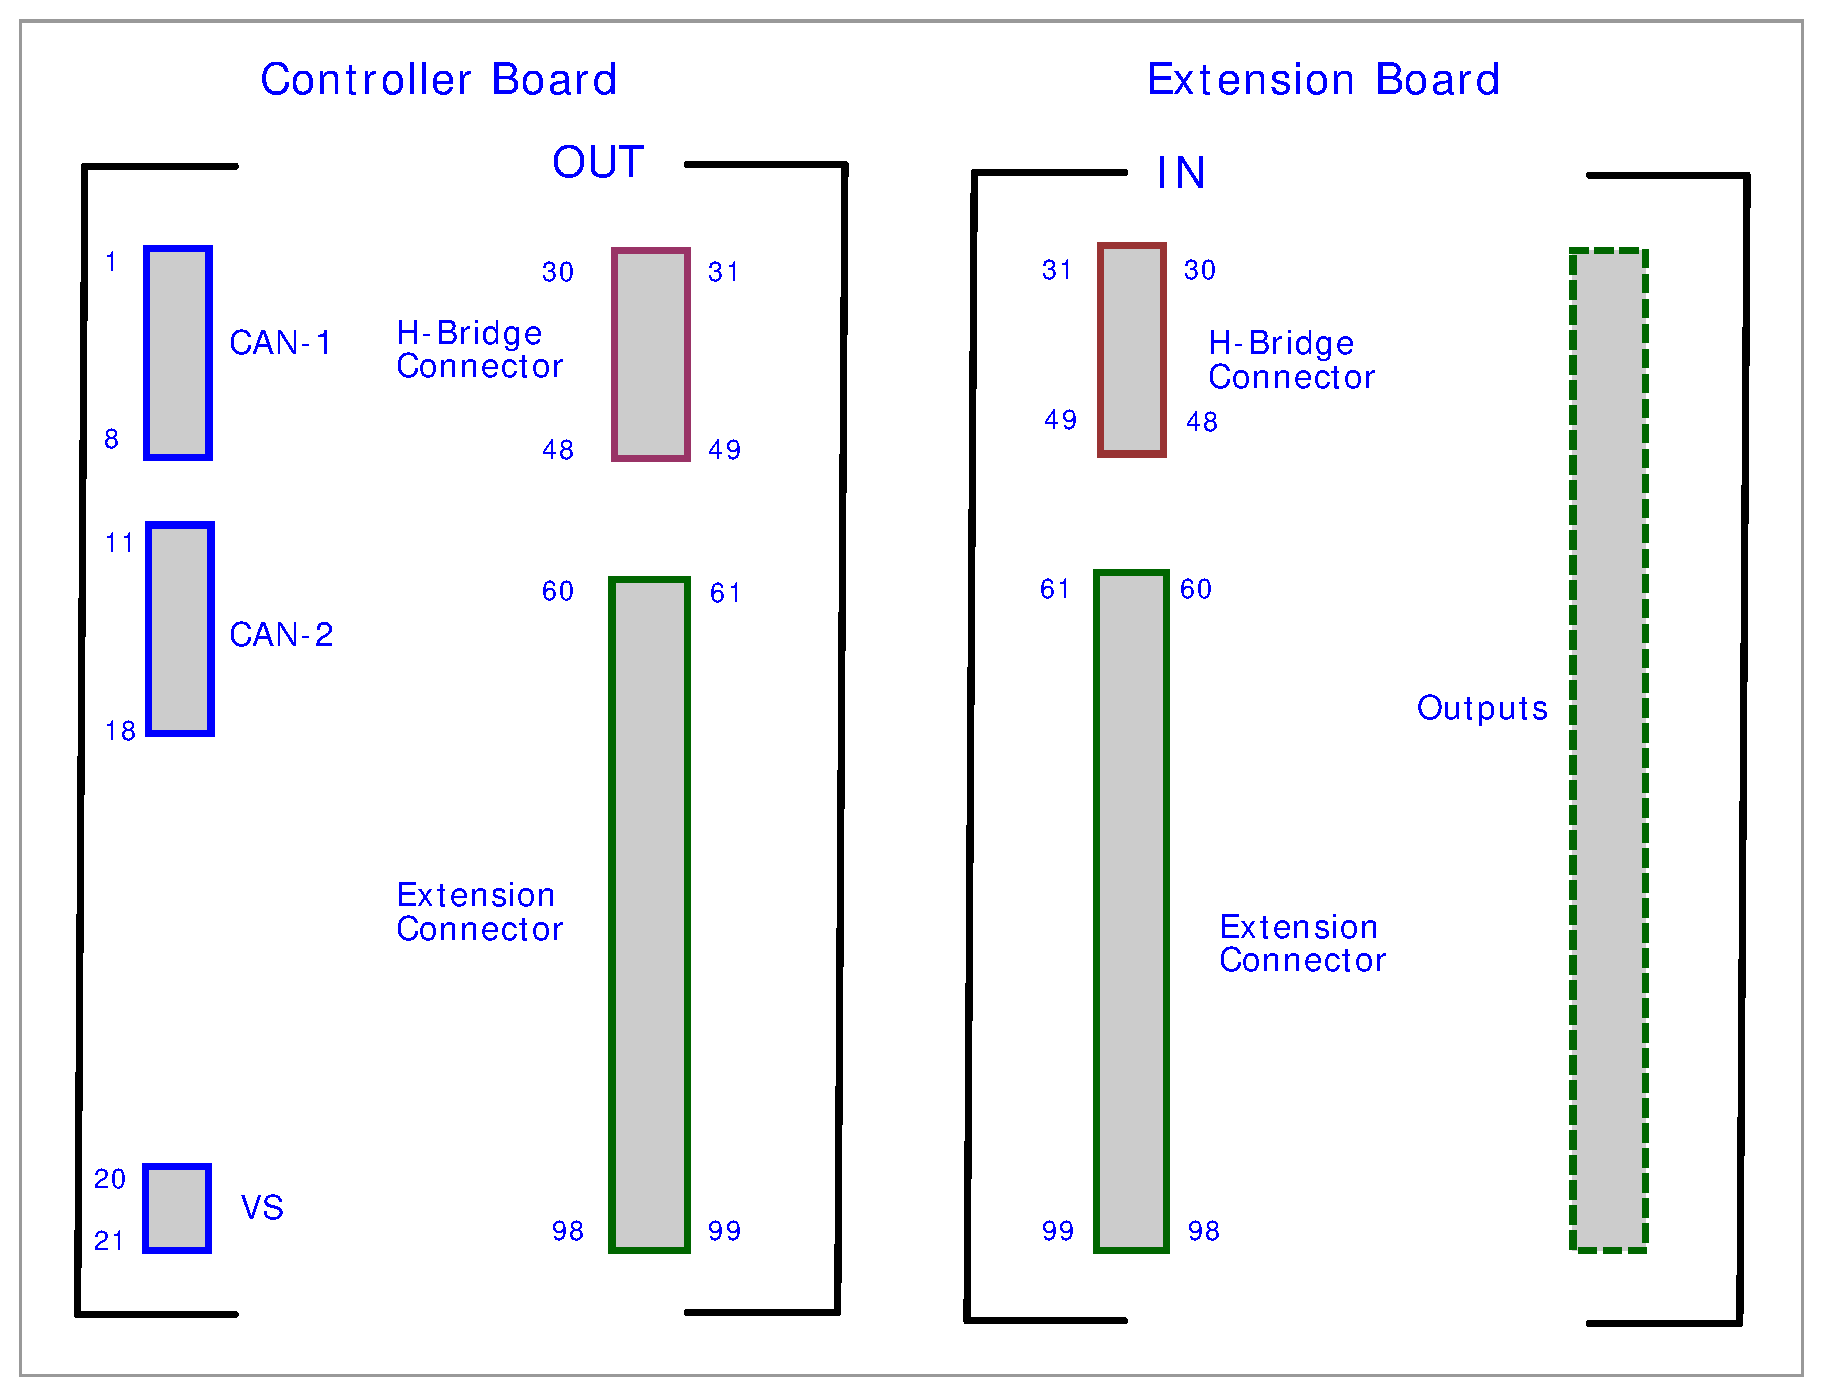
\includegraphics[page=1, scale=0.4]{./Figures/PCB-Connector-Footprint-Pad-Numbers.pdf}
    \caption{PCB-Connector-Footprint-Pad-Numbers}
    %\label{fig:your-label}
\end{figure}

\FloatBarrier

\section{Links}

\begin{table}[!ht]
    \begin{center}
        \caption{...}
        \begin{tabular}{|l|l|p{0.5\textwidth}|}
            \toprule
            \textbf{Tool} & \textbf{Link} & \textbf{Comment} \\
            \midrule
            EasyEDA & http://easyeda.com/de & Design tool for schematics and PCB layouts \\
            \midrule
            JLCPCB & - & PCB board manufactures and parts provider, order from within EasyEDA \\
            \bottomrule
        \end{tabular}
    \end{center}
\end{table}

\input{part-appendix/appendix-inspiring-work-and-links} 
\chapter{Tests}


\section{Pictures}


% example for the protocol chapter... instead of the tables....

\subsection{Protocol boxes}

A bit cumbersome and we would need to have text at defined locations. Perhaps keep the simple table in the protocol chapter.

\begin{center}
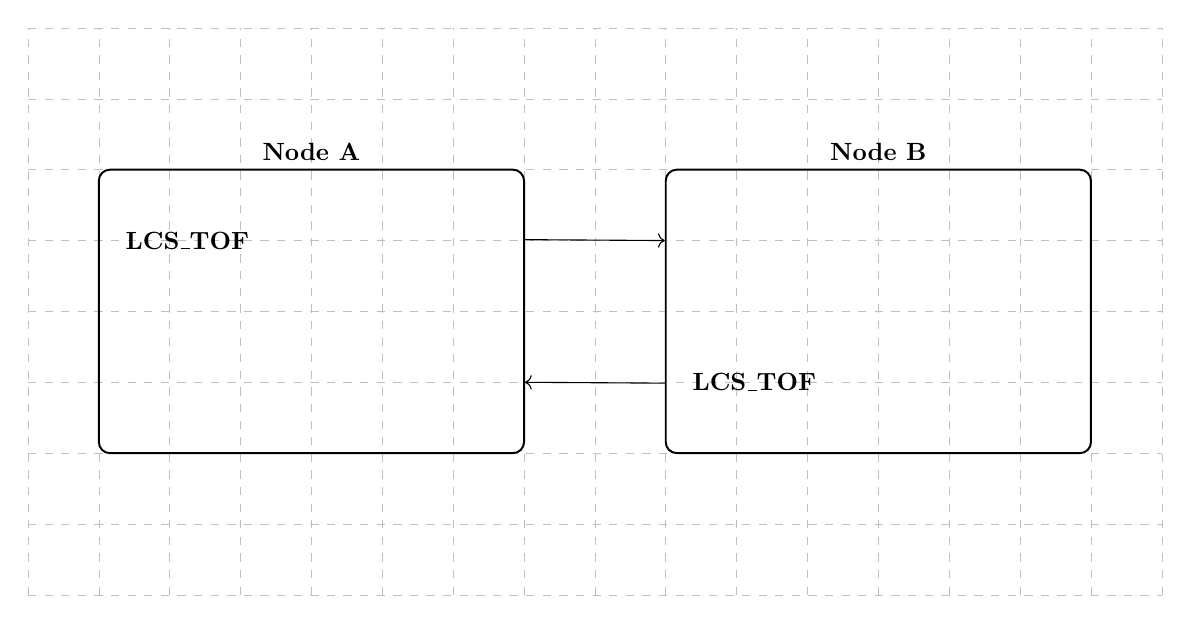
\begin{tikzpicture}[scale=0.9, transform shape]

    \draw[help lines, gray!50, dashed] (0,0) grid( 16,8);

    \node[  draw, 
            tsRoundedRectangle, 
            minimum width=6cm, 
            minimum height=4cm, 
            text height=1cm, 
            align=left] (A) at (4, 4) 
            { };

    \node[  draw, 
            tsRoundedRectangle, 
            minimum width=6cm, 
            minimum height=4cm, 
            text height=1cm, 
            align=left] (B) at (12, 4) 
            { };

    \draw[->] (A.north east) ++(0, -1) -- ($(B.west) + (0, 1 )$);
    \draw[->] (B.south west) ++(0,  1) -- ($(A.east) + (0, -1)$);

    \node at ( 4,  6.25 ) {\textbf{Node A}};
    \node at ( 12, 6.25 ) {\textbf{Node B}};

    \node at ( 2.25,  5 ) {\textbf{LCS\_TOF}};
    \node at ( 10.25, 3 ) {\textbf{LCS\_TOF}};

\end{tikzpicture}
\end{center}


\subsection{Block Node boxes}


% Command: \rectwithports{west count}{east count}{width}{rectID}{x}{y}
\newcommand{\rectwithports}[6]{%
    % #1 = west count, #2 = east count
    % #3 = width, #4 = rectID, #5 = x pos, #6 = y pos
    \pgfmathsetmacro{\nports}{max(#1,#2)}
    \pgfmathsetmacro{\h}{\nports*0.4} % rectangle height

    % Rectangle
    \node[draw, rectangle, minimum width=#3, minimum height=\h cm] (rect#4) at (#5,#6) {};

    % West ports
    \foreach \i in {1,...,#1} {
        \node[circle, draw, fill=green, inner sep=0pt, minimum size=6pt]
            (W#4\i) at ($(rect#4.west) + (0,{(#1-2*\i+1)*0.5*0.4})$) {};
    }

    % East ports
    \foreach \i in {1,...,#2} {
        \node[circle, draw, fill=green, inner sep=0pt, minimum size=6pt]
            (E#4\i) at ($(rect#4.east) + (0,{(#2-2*\i+1)*0.5*0.4})$) {};
    }
}

% Command: \connectports[<TikZ options>]{srcRectID}{srcSide}{srcPort}{dstRectID}{dstSide}{dstPort}
\newcommand{\connectports}[7][]{%
    % Build node names
    \edef\srcnode{#3#2#4}
    \edef\dstnode{#6#5#7}

    % Determine start and end coordinates
    \coordinate (start) at (\srcnode.center);
    \coordinate (end) at (\dstnode.center);

    % Adjust start/end to the correct side of the port
    \ifthenelse{\equal{#2}{E}}{\coordinate (start) at (\srcnode.west);}{\coordinate (start) at (\srcnode.east);}
    \ifthenelse{\equal{#5}{E}}{\coordinate (end) at (\dstnode.east);}{\coordinate (end) at (\dstnode.west);}

    % Draw orthogonal line (Manhattan style)
    \draw[-, #1] (start) -- (end);
}



\begin{tikzpicture}
  % Draw rectangles
  \rectwithports{2}{2}{2cm}{1}{0}{0}    % rectID=1 at (0,0)
  \rectwithports{3}{1}{4cm}{2}{6}{0}    % rectID=2 at (6,0)
  \rectwithports{3}{1}{4cm}{3}{12}{0}   % rectID=3 at (12,0)

  % Connect ports
  \connectports[->, red, thick]{1}{E}{1}{2}{W}{2}   % rect 1 E1 -> rect 2 W2
  \connectports[->, blue, thick]{2}{E}{1}{3}{W}{1}  % rect 2 E1 -> rect 3 W1
\end{tikzpicture}



   
% \include{appendices/LCS-Item-Reference}
% \include{appendices/LCS-Command-Reference}
% \include{appendices/DCC-PP-Command-Reference}
% \chapterr{\textit{Appendix n - Runtime Library Routines Reference}}

// ??? \textbf{note} this appendix will not repeat what is documented in the source. This is a battle you cannot win. I have a small utility that takes an augmented C-source include file and makes it a markdown document. 

// ??? \textbf{note} we could just include this file, or keep a reference to it for the utility to include. The result of the utility is a markdown file with all the text in this file and the included files, which is then the base for PDF creation.

// ?? \textbf{note} have a table with all items... 

| Item | purpose | Get | Put | Req |
|:--|:--|:--:|:--:|:--:|
| an item | what it does | X | X | - |
% ## *Appendix n - Controller Dependent Code Library Routines Reference*

// ??? **note** this appendix will not repeat what is documented in the source. This is a battle you cannot win. I have a small utility that takes an augmented C-source include file and makes it a markdown document. 

// ??? **note** we could just include this file, or keep a reference to it for the utility to include. The result of the utility is a markdown file with
// all the text in this file and the included files, which is then the base for PDF creation.

% ## *Appendix n - A generic power supply*

Depending on the actual node hardware design, power is implemented in a variety of ways. A small handheld node would certainly draw its power from the LCS bus. A booster has a much higher power consumption requirement. The typical node needs in any case a 5V power, which can for example be drawn from a high power line on the layout. And as with every building block shown so far, there are many ways to Rome.

A power supply for a generic node could draw power from the LCD bus or from an external power line. Furthermore, some LCS nodes need a way to detect a power failure and perform any last second items before power is gone. The following schematic shows a power supply that allows for automatic switching between two inputs. It also features a power fail detection mechanism.


![Schematic_LcsNodes-Building-Block-Generic-Power-Supply.png](./Schematics/Schematic_LcsNodes-Building-Block-Generic-Power-Supply.png )

The right part of the schematic shows how the power input lines are switched depending what is connected. The voltage regulator itself is pretty much standard. Since the power line may have up to 24Volts, a switched regulator is a good choice. The right side features a power fail signal detection output and a capacitor to provide power for the last actions before power done. Naturally the timing depends on the actual power drawn by the board. When a power fail is detected, it is a good idea to immediately turn off power consuming devices and focus on the last items to do before power is gone. A good example is to save the last data items in the non-volatile storage.
% \include{appendices/appendix-lcs-guidance-computer}

    %--------------------------------------------------------------------------------
%
% 
%--------------------------------------------------------------------------------
\part{LCS Listings}

% \iftoggle{includeListings}{ \chapter{Listings test}

Here is a little test how a listing part might be shown ...

\lstset{style=listingstyle}
\lstinputlisting[language=c++]{./listings/main.cpp}
 }

    
    %----------------------------------------------------------------------------    
    % Back matter (table of contents, etc.)
    %----------------------------------------------------------------------------
    \backmatter    
    \printindex         

\end{document}
